%!TEX root = ../Hardtung_BA_SoSe20.tex

\section{Planning Solutions}
\label{sec:planningSolutions}

This section will build on the discovered usability issues found during the initial evaluation process (see \ref{sec:evaluation}). On this basis, first solutions can be planned that fix the most impactful usability issues. Furthermore, new features can be developed that increase productivity (by automating processes and part of the workflow), while also fixing the current problems.


\subsection{Graphical User Interface related changes}

These changes include everything that is related to the graphical user interface that the user interacts with.

\subsubsection{Overall UI Changes}
Every feature area (e.g. grid options, scaling options, arrow/symbol inputs etc.) should be seperated through a \texttt{EtchedBorder} with its name as the title. Within these borders, elements should follow a consistent order. This is why this hierarchy is being set for the placement within these areas: \texttt{JRadioButton, JTextField, JButton, JCheckBox}.

Though additional \texttt{JLabels} can be used to explain or to give indicators what the elements do specifically. Whenever possible, icons should replace text and tooltips should be used to give further explanation. Explanatory \texttt{JLabels} should only be used when icons and tooltips are not enough.

Additionally to the more consistent placement of elements within the UI, their sizes should be standardized as well. \texttt{JTextFields} for example should only be large enough to encapsulate the largest possible entry. This means that the \texttt{height} should always be set to 25 pixels ( and the \texttt{width} depending on what is being entered (e.g. entering an angle between 0-360° will be shorter than entering the textual explanation of a folding step).
\newline
\textbf{Fixes: 02; 04; 21; 22; 23}\\
\newline
%Later Change
At a later point a complete redesign and rework of the UI will have to be carried out, in order to facilitate the goal of a unified and obstructionless design. At the current stage of development though the focus is being set to increase the efficiency and speed of creating origami diagrams, as this is the main reason why the Origrammer exists.

\subsubsection{Arrows \& Symbols}
A large part of the Origrammer is made up of the different arrows and symbols that can be used in diagrams. So far, these objects were simple vector graphics that were being placed on the diagram as \texttt{ImageIcons} of \texttt{JLabels}. This approach did initially work, but brought restrictions and problems with it.

 As vector graphics do not have explicit width or height values, the library Batik\cite{batik}, which was being used to load the .svg files, presented wrong values to the \texttt{JLabel.setBounds(width, height)}-method. As a result of this limitation, the arrows \& symbols got partially cut off at the original bounds of the \texttt{JLabel} when rotating them. To fix this issue, a new, pre-rotated vector graphic was being loaded whenever an arrow or symbol got rotated. Though this in turn facilitated itself in a wrong, always square border around the arrows and symbols. Additionally, this made interactions with arrows and symbols far slower and unflexible.
 
 Another sideeffect was a change in scale when rotating a non square object. The \texttt{JLabel} tries to display the biggest possible object that can fit within the border bounds. As seen on Figure \ref{fig:unwantedScaling} the size of the arrow changes after rotating it by 45°.

\begin{figure*}[htbp]
	\centering
	\begin{subfigure}{0.3\textwidth}
		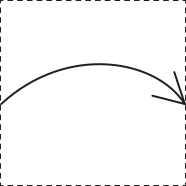
\includegraphics[width=\textwidth]{arrowLabelBorderStraight}
		\caption{Straight Arrow}
		\label{fig:arrowLabelBorderStraight}
	\end{subfigure}
	\begin{subfigure}{0.3\textwidth}
		\includegraphics[width=\textwidth]{arrowLabelBorderAngled}
		\caption{Angled Arrow}
		\label{fig:arrowLabelBorderAngled}
	\end{subfigure}
	\caption{Unwanted Scaling when Rotating}
	\label{fig:unwantedScaling}
\end{figure*}

As a result of all these problems and limitations, the decision was made to completely rework how arrows \& symbols function in the Origrammer. The new approach was to rebuild all objects with simple \texttt{java.awt.Shape}-objects. This gave total control over rotations, scaling, and on-the-fly-editing of all arrows/symbols. Another advantage was the removed reliance on \texttt{JLabels} and associated with that, there were no longer issues with wrong hitboxes or different scaling while rotating. The only disadvantage was the work-intensive nature of remodeling all arrows and symbols with \texttt{Shape}-objects by hand.
\newline
\textbf{Fixes: 15; 25; 26}
\subsubsection{Side Panel}

The text of the \texttt{JRadioButtons} at the tool bar should be replaced by self-explanatory icons in order to improve overall clarity. But the textual explanation of all the tools should still be present to help especially novizes. This can be done through tooltips that appear when hovering over the buttons.

\textbf{Fixes: 02; \emph{22}}

\subsection{User Input related changes}

\subsection{New Origrammer features}

These new features should increase the productivity and efficiency of the Origrammer. The focus should be set on maximising the work that can be done in the shortest amount of time. This will be achieved by implementing features that either automate parts of the workflow, or that give new, faster possibilities of achieving the goal.